\documentclass[a4paper, 12pt ]{article}
\usepackage{graphicx}
\usepackage{geometry}
\geometry{margin=1in}
\usepackage{multicol}
\usepackage{wrapfig}
\usepackage[rightcaption]{sidecap}
\usepackage{todonotes}


\author{Laura Puente-Santamaria, Luis del Peso}
\title{TFEA.ChIP\\\large A tool kit for transcription factor binding site enrichment analysis capitalizing on ChIP-seq datasets}

\begin{document}
	\maketitle
\begin{abstract}

The identification of transcription factor (TF) responsible for the co-regulation of an specific set of genes is a common problem in transcriptomics. With the development of TFEA.ChIP we aim to provide a tool to estimate and visualize TF enrichment in a set of differentially expressed genes that takes into account the wide variation in TF's behavior across different cell types and stimuli. To that end, ChIP-Seq experiments from the ENCODE Consortium and GEO Datasets were gathered, and a database linking TFs with the genes they interact with in each ChIP-Seq experiment was generated. In its current state, TFEA.ChIP covers 333 different transcription factors in 1122 ChIP-Seq experiments, with over 150 cell types being represented.
\todo[size=\tiny, backgroundcolor= yellow!50 ]{Include here comparison with Opossum and results.}

\end{abstract}

\section{Introduction}

 In the most simple scenario, the comparison of the transcriptome of cells or organisms in two conditions leads to the identification of a set of differentially expressed (DE) genes, and the underlying assumption is that one or a few TFs regulate the expression of those genes. Traditionally, the identification of relevant TFs has relied on the use of position weight matrices (PWMs) to predict transcription factor binding sites (TFBSs) proximal to the DE genes\cite{Wasserman}. The comparison of predicted TFBS in DE versus a set of control genes, reveals factors that are significantly enriched in the DE gene set. The prediction of TFBS using these approaches have been useful to narrow down potential binding sites, but can suffer from high rates of false positives. In addition, this approach is limited by design to sequence-specific transcription factors (TF) and thus unable to identify cofactors that bind indirectly to target genes. To overcome these limitations we developed the R package TFEA.ChIP, which exploits the vast amount of publicly available ChIP-Seq datasets to determine TFBS proximal to a given set of genes and computes enrichment analysis based on this experimentally-derived rich information. Specifically TFEA.ChIP, uses information derived from the hundreds of ChIP-Seq experiments from the ENCODE Consortium\cite{ENCODE} expanded to include additional datasets contributed to GEO database\cite{GEO1}\cite{GEO2} by individual laboratories representing the binding sites of factors not assayed by ENCODE. The package includes a set of tools to customize the ChIP data, perform enrichment analysis and visualize the results. Herein we describe the main characteristics of the package and compare the results produced by TFEA.ChIP vs those generated by Oppossum, an state of the art TFBS identification software based on PWMs \cite{Kwon2012}. Our data indicate that the results of TFEA.ChIP and Opossum are coincident for those datasets where Oppossum identifies clear TFBS candidate(s). In addition, TFEA.ChIP identified enriched factors for some data sets where Opossum was unable to find a significant match.\todo[size=\tiny, backgroundcolor= yellow!50 ]{Indicate that the factors found by TFEA.ChP are the ones expected according to the experimental manipulations in each dataset.}
 
 \todo[size=\tiny, backgroundcolor= yellow!50 ]{I would move the following paragraphs to results.}
 The package implements two enrichment analysis methods:

\begin{itemize}
 \item Analysis of the association of TFBS and differential expression from 2x2 tables recording the presence of binding sites for a given TF in DE and control genes. The statistical significance of the association for each factor determined by a Fisher’s exact test.
 
 \item GSEA analysis, based on the core function of the GSEA algorithm for R\cite{GSEA1}\cite{GSEA2}, GSEA.EnrichmentScore.
\end{itemize}

TFEA.ChIP includes a TF-gene interaction database containing 1122 datasets from ChIP-Seq experiments testing 333 different human transcription factors. Although the package is mainly focused towards analyzing expression data generated from human cells, TFEA.ChIP includes the option to use datasets coming from experiments in mice, translating mouse gene names to their equivalent ID on the human genome. 
\todo[size=\tiny, backgroundcolor= yellow!50 ]{Adding mention to web implementation if done.}

\section{Building our TFBS database}

\begin{wrapfigure}{r}{0.55\textwidth}
	\centering
	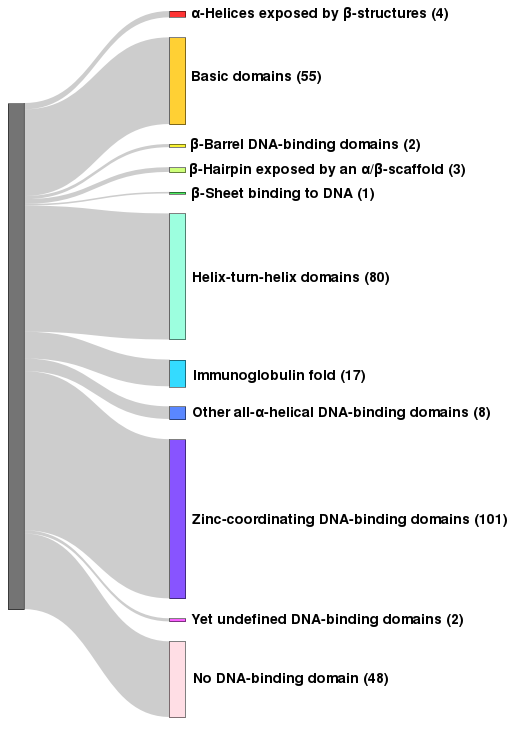
\includegraphics[width=0.5\textwidth]{superclases}
	 \caption{Structural diversity according to DNA binding domains of the 333 transcription factors included in the TFBS database.}
\end{wrapfigure}

The first source of ChIP-Seq datasets is Encode Uniform TFBS database, which guarantees a standard procedure to gather, filter, and share information from ChIP-Seq experiments. However, taking into consideration that the current estimations of the amount of transcription factors in the human genome range from 1,391\cite{TFcensus} -manually curated candidates- to 2886 -predicted through computational methods by DBD\cite{DBD1}\cite{DBD2} -, the 157 transcription factors covered by Encode’s database were not considered enough to build a comprehensive TF enrichment analysis tool.
In order to expand the scope of our TFBS database, we also included datasets from ChIP-Seq experiments stored in GEO. In total, 1122 ChIP-Seq datasets, 689 from Encode and 433 from GEO DataSets, make up the source of information to generate this database, covering 333 different transcription factors in a variety of cell types and experimental conditions.
The process to establish a link between a peak in a ChIP-Seq experiment and a specific gene goes as follows:

\begin{enumerate}
	\item Generating a Dnase Hypersensitive Sites database, linking each Dnase HS to the nearest gene of those included in UCSC Known Gene database\cite{KnownGene}. During this process, DHSs that were farther than 1Kb from any gene were discarded, so as to avoid highly uncertain connections that would undermine the robustness of any analysis. In the case of a DHSs close enough to more than one gene, both were assigned to the site. For this purpose we used Encode’s  Master DNaseI HS database\cite{EncodeDHS1}\cite{EncodeDHS2}.

	\item Selecting from each ChIP-Seq dataset those peaks that overlap a DHSs. Each of these peaks will be assigned the same gene as the DHS they overlap.
	
	\item Storing the list of genes assigned to a peak in each of the ChIP-Seq experiments. With this lists we generated a binary matrix which rows correspond to all the human genes in the Known Gene database, and its columns, to every ChIP-Seq experiment; the values assigned are 1 –for a peak assigned to that gene – or 0.
	
\end{enumerate}
\begin{figure}[h]
	\centering
	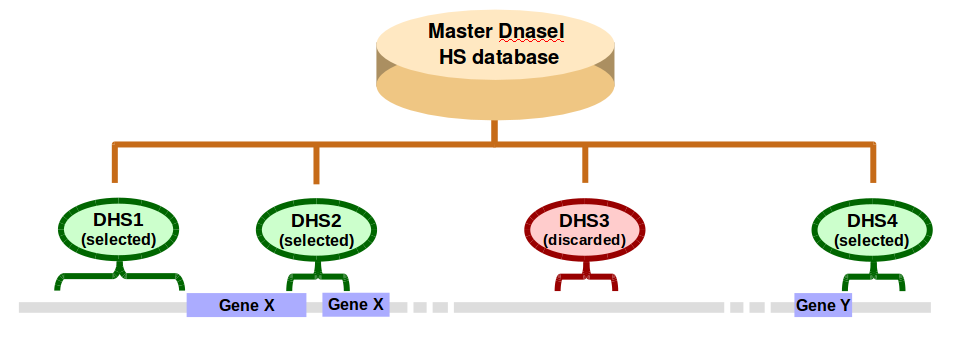
\includegraphics[width=0.8\textwidth]{graf-dhs}
	\caption{Building a DHS database. From Encode’s Master DNaseI HS database, that gathers all DHSs found in several cell lines, we selected those DHSs that are 1Kb or closer to a gene according to the gene’s location on UCSC’s Known Gene database. DHS further than 1Kb from any gene are discarded to avoid highly uncertain links.
	In this illustration, both DHS1 and DHS2 would be assign to gene “X”, and DHS4 to gene “Y”, while DHS3 would be discarded.}
\end{figure}

\begin{SCfigure}[1][h]
	\centering
	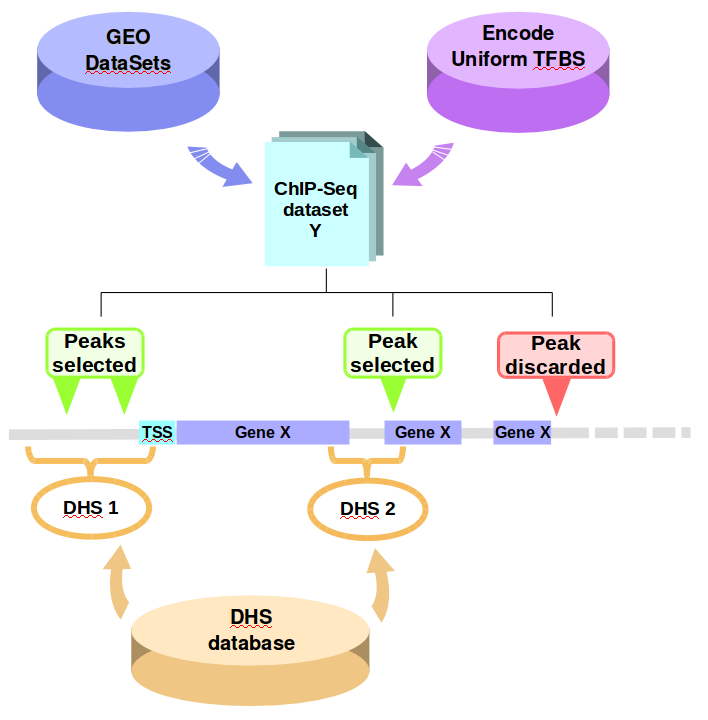
\includegraphics[width=0.45\textwidth]{graf-TFBS_building}
	\caption{Building the TFBS database. For every peak in a ChIP-Seq dataset is tested whether it overlaps any of the DHSs located close to a gene. If the result is positive, the gene corresponding to said DHS –gene “X” in this illustration– will be assigned to the ChIP-Seq experiment, if its negative, that peak will be discarded.
	The ChIP-Seq dataset “Y” has three peaks that overlap DHS1 and DHS2, so the Entrez ID of gene “X” would be associated to the ChIP-Seq “Y”.}
\end{SCfigure}

\section{Analyzing TF enrichment with TFEA.ChIP}

TFEA.ChIP is designed to take the output of a differential expression analysis and identify transcription factors enriched in the list of differentially expressed genes. The core premise of our method is that key effectors of a regulatory response will have more target genes among the differentially expressed than among the unresponsive genes.
In the case of analysis of association, the only required input is a set of DE genes and, optionally, a set of control genes whose expression is not altered by the experimental conditions under the study. 
For the GSEA analysis a ranked list of genes is required. This is supplied as a matrix or data frame containing a column with gene names and a numerical column with the ranking metric, which typically are log2(Fold change) for the gene expression changes in the two conditions under evaluation. 

\subsection{Association analysis}

The simplest approach to transcription factor enrichment consist on comparing how many targets of a given transcription factor are in two lists of genes. This is the course of action taken in this method, focused on finding differences in transcription factor enrichment between differentially expressed genes (be it up-regulated, down-regulated or both) and a control group. To that end, the program generates contingency matrices for every ChIP-Seq experiment in the database, estimating statistical significance using Fisher's exact test is performed.

\begin{SCfigure}[1][h]
	\centering
	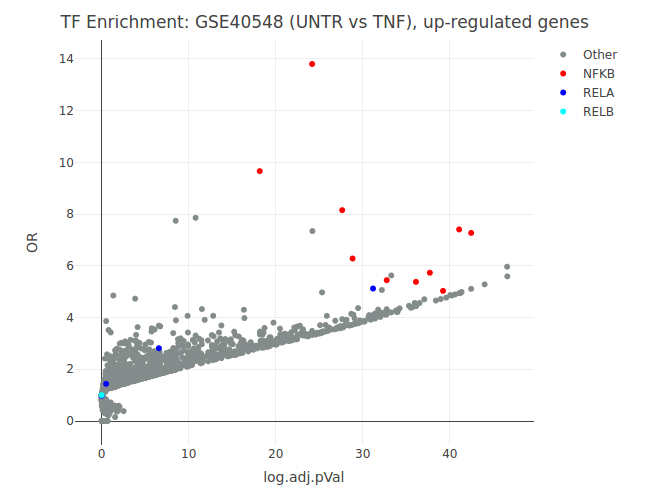
\includegraphics[width=0.50\textwidth]{graf-tfea1}
	\caption{Association analysis performed on up-regulated vs un-responsive genes in neutrophils after TNF addition. As expected, the main enriched TF -NFK$\beta$ and RELA- are related with inflammatory processes.}
\end{SCfigure}

\subsection{GSEA-like analysis}

This method is based on the same principle than GSEA\cite{GSEA1}\cite{GSEA2}: having the list of genes of an RNA-seq experiment ordered by log2(Fold Change), for every ChIP-Seq in the database, the algorithm starts by calculating how many matches and mismatches there are between the gene list provided and the genes associated to each ChIP-Seq experiment in the database. With the amounts of matches and mismatches, it generates a match score and a mismatch score, so that Enrichment Score is always delimited between 1 and -1. The result is an array in which every time a gene in the list provided is associated to the ChIP-Seq experiment, the match score is added, while on the rest of cases, the mismatch score is subtracted -Running Enrichment Score or \textit{RES}. The final Enrichment Score given to each experiment is the absolute maximum of the RES.

\begin{figure}[h]
	\centering
	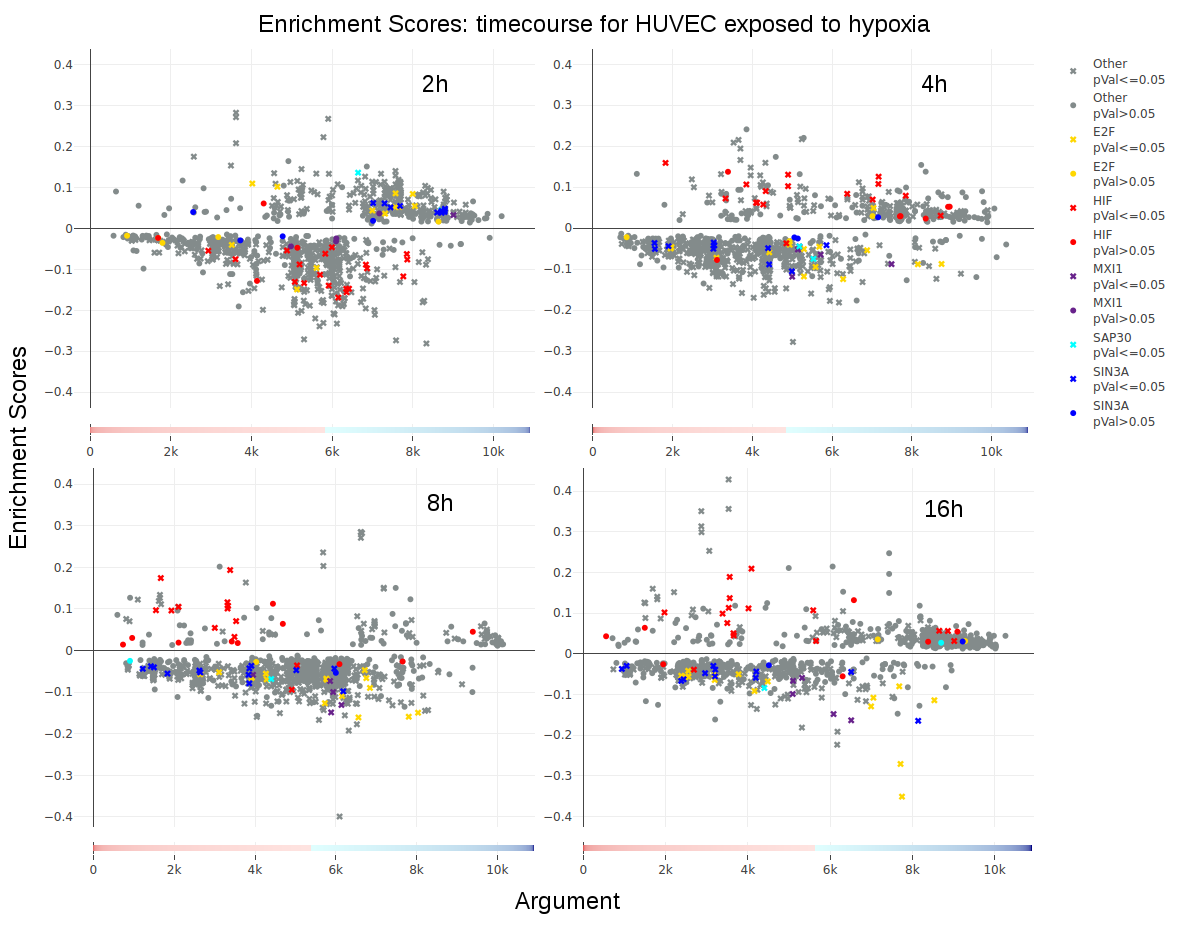
\includegraphics[width=\textwidth]{graf-tfea2}
	\caption{GSEA-like analysis of gene expression on HUVEC exposed to hypoxia vs normoxia at several times. As is shown in the figure, HIF-mediated response to hypoxia starts at 4h, and reaches it's peak at 8h, when most of it's targets are among up-regulated genes. The same pattern of behavior can be observed in repressors, that reach their maximum enrichment among down-regulated genes between 8 and 16h after exposure.}
\end{figure}

\begin{SCfigure}[0.9][h!]
	\centering
	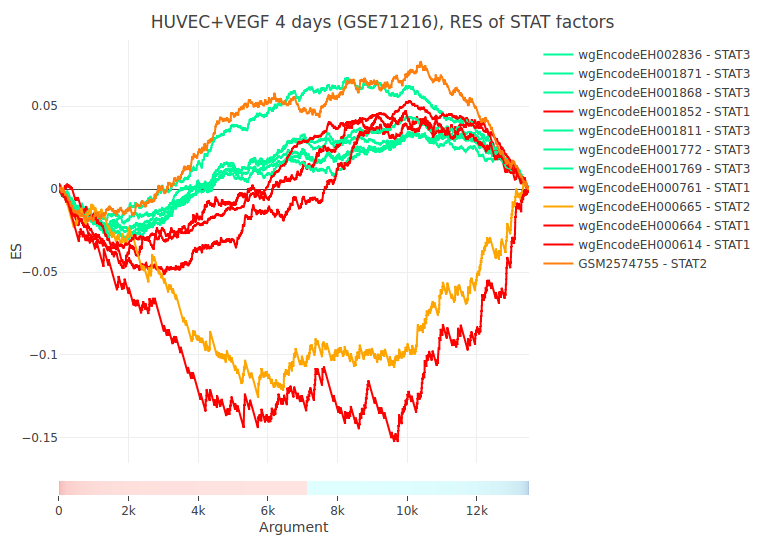
\includegraphics[width=0.55\textwidth]{graf-tfea3}
	\caption{plot of the Running Enrichment Score in an RNA-seq experiment on HUVEC cells supplemented with VEGF for 4 days for STAT1, STAT2 and STAT3 ChIP-Seqs.
	The ChIP-Seqs wgEncodeEH000664 and wgEncodeEH000665 were done with a IFNα treatment while the rest of STAT1 and STAT2 ChIPs were done using IFNγ. Since IFNα is a known angiogenesis inhibitor, the targets of this two ChIPs are significantly different than those of the ChIPs done with IFNγ, and in this case, amongst the down-regulated genes.}
\end{SCfigure}


\section{Comparison with similar software: oPOSSUM's single site analysis}

To test TFEA.ChIP's performance, we decided to compare its TF enrichment estimations with a program that uses a related approach to measuring TF enrichment: oPOSSUM's Single site analysis (SSA)\cite{opossum}. In contrast with our package, oPOSSUM's SSA searches for potential TF binding sites in the sequences of a given set of genes compared to a background set.

Several validation sets were used, mainly focusing on upregulated vs. unresponsive genes
(with one case of downregulated vs. unresponsive genes during hypoxia). These validation
sets include:
\begin{itemize} \itemsep-0.5em
	\item Hypoxia vs normoxia in HUVEC cells.
	\item TNF addition in neutrophils and adipocytes.
	\item Left ventricular non-compaction in cardiomyocytes.
	\item INFα addition in hESC cells for 15 and 21 days.
\end{itemize}

To compare both methods we generate contingency matrices with the number of target
hits, target non-hits, background hits, and background non-hits for every profile and ChIP- Seq experiment, and then performed Fisher’s exact test. The resulting p-values are
adjusted for multiple testing using FDR method.

\subsection*{Hypoxia vs normoxia in HUVEC cells}

oPOSSUM 3.0 it’s limited by design to transcription factors that bind directly to a specific DNA sequence, so important cofactors during hypoxia, like SIN3A, that don’t have a DNA binding domain, are excluded from the analysis. Since the source of information for TFEA.ChIP are ChIP-Seq experiments, we’re able to collect binding information for TFs that aren’t sequence specific or depend on other cofactors to function.

Using significantly up-regulated genes, both TFEA.ChIP and oPOSSUM are able to detect and enrichment in ARTN targets, but TFEA.ChIP also detects significant enrichment in HIF1A, EPAS1, and EZH2. The last transcription factor is part of a histone modification complex, and doesn’t bind directly to DNA, so is not included in oPOSSUM’s database.
\begin{SCfigure}[0.7][h]
	\centering
	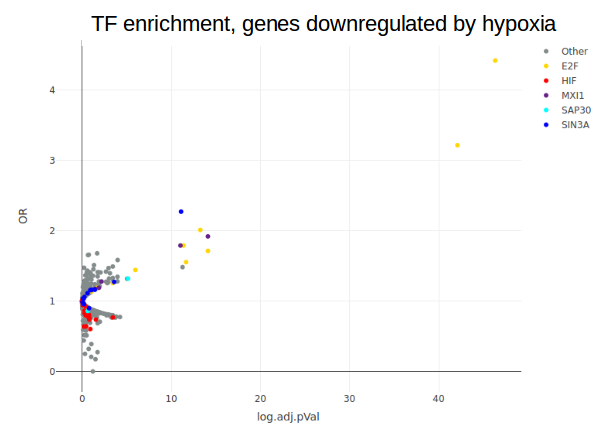
\includegraphics[width=0.55\textwidth]{graf-op1}
	\caption{For down-regulated genes, after adjusting p-values, oPOSSUM doesn’t find any TF significantly enriched, while TFEA.ChIP detects significant enrichment in 111 different TFs, being the most important E2F4, E2F7, SIN3A, MXI1, and E2F1.}
\end{SCfigure}


\subsection*{TNF addition in neutrophils and adipocytes}
In case of genes upregulated by TNF addition, both oPOSSUM and TFEA.ChIP are able to detect a significant enrichment in NfκB, REL and between 5 and 20 more TFs –depending on the experiment–. Most of the transcription factors detected only by one of the methods are not included in the other one’s database. This shows that, when a transcription factor’s response doesn’t change much depending on stimuli or tissue, both methods perform similarly.

\subsection*{Left ventricular non-compaction in cardiomyocytes}
In a complex case, such as left ventricular non-compaction, both methods are able to detect a significant enrichment in HIF factors –as expected, since LVNC is associated to hipoxemic conditions– along with another 17 significantly enriched or depleted factors.
Of the 71 TF enriched TFs detected by oPOSSUM, 29 are not in TFEA.ChIP’s database, while the same happens with most of the enriched transcription factors detected by TFEA.ChIP, such as KDM3A or EZH2.

\begin{figure}[h]
	\centering
	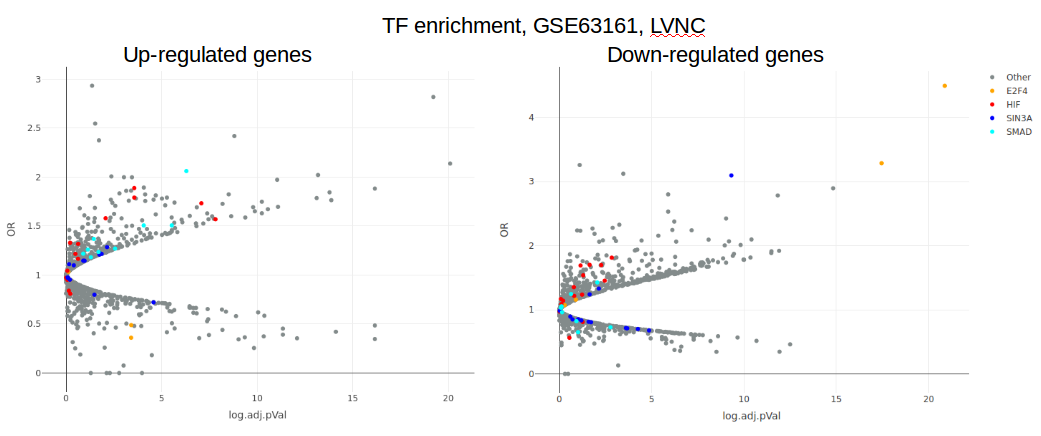
\includegraphics[width=\textwidth]{graf-op2}
	\caption{Enrichment analysis in LVNC. TFEA.ChIP is able to find several enriched TF. Some of the most important are HIF factors (in red) along with SMAD2, SMAD4 (cyan) and E2F4 (yellow), while SIN3A only has one ChIP-Seq experiment among those highly	enriched.}
\end{figure}

\subsection*{INFα addition in hESC cells for 15 and 21 days}
As previous studies have concluded\cite{geneReg}, regulation networks can differ greatly depending on the tissue and the stimuli applied. An example of this behavior would be Signal Transducer And Activator Of Transcription –STAT– factors, such as STAT1 Or STAT2, whose targets change depending on the interferon type used as stimulus. This behavior can be seen in figure \ref{fig6}.
\newline
\newline
\newline

\begin{SCfigure}[1][h]
	\centering
	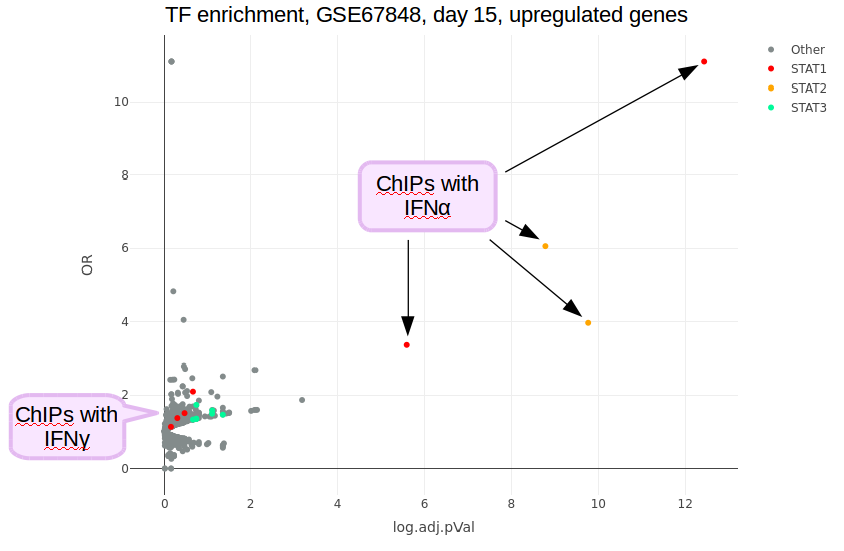
\includegraphics[width=0.65\textwidth]{graf-op3}
	\caption{Validation dataset GSE67848, hESC + IFNα, day 15, upregulated genes.  Two of the STAT1 ChIP-Seq experiments and the STAT2 ones were done after IFNα addition while the rest of STAT1 ChIPs were treated with IFNγ. In both association analysis and GSEA-like analysis, TFEA.ChIP is able to detect conditional TF enrichment.}
	\label{fig6}
\end{SCfigure}


\subsection*{Conclusion}
In general, TFEA.ChIP allows to take into account cellular context (tissue, stimuli) on which an expression experiment is done, making possible to detect enrichment in transcription factors in cases where oPOSSUM can’t, due to:
\begin{itemize}
	\item Indirect binding: in case of complexes such as the Polycomb Repressive Complex or SIN3A, that is a co-factor of MXI1.
	\item Stimuli-dependent binding: as seen previously with STAT and IRF factors.
\end{itemize}


On another note, oPOSSUM allows the user to have more control over some of the parameters used for the analysis (conservation cutoff or matrix score threshold, for instance) while TFEA.ChIP analysis only takes as input two lists of genes. More over,since TFEA.ChIP’s sources are treatment and tissue specific, in some cases the result
might not be applicable to the dataset used as input (i.e., tissues or cell types that have a very particular regulatory pattern, when there are no ChIP-Seq experiments done in said cell type).

\section{Dependencies and requirements}
The following R packages are used to run TFEA.ChIP:
\begin{enumerate} \itemsep-0.5em
	
	\item Packages part of Bioconductor\cite{bioconductor}:
	\begin{itemize} \itemsep-0.5em
		\item GenomicRanges, IRanges, and GenomicFeatures\cite{GRanges}
		\item biomaRt\cite{biomart1}\cite{biomart2}
		\item TxDb.Hsapiens.UCSC.hg19.knownGene\cite{TxDb.knownGene}
		\item org.Hs.eg.db[19]
	\end{itemize}

	\setcounter{enumi}{4}
	\item plotly\cite{plotly}
	\item dplyr\cite{dplyr}
	\item knitr\cite{knitr}
	\item rmarkdown\cite{rmarkdown}
	\item S4Vectors\cite{S4Vectors}
	\item scales\cite{scales}
\end{enumerate}
\todo[inline, backgroundcolor = orange!50, caption={R version and web implementation}]{I'll add here what R version the package runs on (currently in Bioconductor's development version is R $\geq$ 3.5, but in the release branch is usually a lower version). \newline If a web implementation it's done it will be mentioned here to.}


\bibliographystyle{unsrt}
\bibliography{borrador_paper}

\listoftodos

\end{document}

@article{ID,
	author = {author},
	title = {title},
	journaltitle = {journaltitle},
	date = {date},
}
